\chapter{Martingales in diskreter Zeit}

% ============================================
% BOSS CHALLENGE - Dark Souls Style
% ============================================
\begin{bosschallenge}[Der Martingal-Dämon]
\textbf{Schwierigkeitsgrad:} $\star\star\star\star\star$ (Extrem)

\textbf{Name des Bosses:} Der Martingal-Dämon von diskreter Zeit

\textbf{Herausforderung:}

Sei $(\Omega, \mathcal{F}, \mathbb{P})$ ein Wahrscheinlichkeitsraum und $\{\mathcal{F}_n\}_{n \geq 0}$ eine Filtration. Betrachten Sie eine Folge von Zufallsvariablen $\{X_n\}_{n \geq 0}$, die an $\{\mathcal{F}_n\}$ adaptiert ist.

\textbf{Problem:} Beweisen Sie, dass wenn $\{X_n\}$ ein Martingal ist und $\tau$ eine Stoppzeit mit $\mathbb{E}[\tau] < \infty$ ist, dann gilt:

\begin{align}
\mathbb{E}[X_\tau] = \mathbb{E}[X_0]
\end{align}

\textbf{Zusätzliche Herausforderung (NG+ Modus):} Zeigen Sie, dass diese Aussage im Allgemeinen \textit{falsch} ist, wenn man die Bedingung $\mathbb{E}[\tau] < \infty$ entfernt. Konstruieren Sie ein Gegenbeispiel.

\textbf{Hinweise:}
\begin{itemize}
    \item Verwenden Sie das Optional Sampling Theorem (das Sie in diesem Kapitel lernen werden)
    \item Denken Sie an die Bedingungen für gleichgradige Integrierbarkeit
    \item Betrachten Sie ein einfaches symmetrisches Random Walk als Beispiel
\end{itemize}

\textbf{Bonus-Quest:} Wenn Sie diese Herausforderung lösen, haben Sie bereits die tiefsten Geheimnisse der Martingal-Theorie verstanden!

\vspace{0.5cm}
\textit{"In der Welt der Stochastik gibt es keine Gnade. Nur Martingale und ihre Eigenschaften."}
\end{bosschallenge}

\vspace{1cm}

% ============================================
% DENOOBIFICATION - Grundbegriffe
% ============================================

\section{Denoobification: Grundlegende Begriffe}

Bevor wir mit Martingalen beginnen, müssen wir sicherstellen, dass alle grundlegenden Begriffe klar sind. Dieser Abschnitt erklärt die wichtigsten Konzepte für Anfänger.

\begin{denoobification}[Wahrscheinlichkeitsraum]
\textbf{Was ist ein Wahrscheinlichkeitsraum?}

Ein \textbf{Wahrscheinlichkeitsraum} ist das fundamentale mathematische Modell für Zufallsexperimente. Er besteht aus drei Komponenten:

\begin{enumerate}
    \item \textbf{$\Omega$ (Omega) - Ergebnismenge:} Die Menge aller möglichen Ergebnisse eines Zufallsexperiments.
    
    \textbf{Beispiel:} Beim Werfen eines Würfels ist $\Omega = \{1, 2, 3, 4, 5, 6\}$.
    
    \item \textbf{$\mathcal{F}$ (F) - $\sigma$-Algebra:} Eine Sammlung von Teilmengen von $\Omega$, die die "messbaren Ereignisse" beschreibt. Sie muss folgende Eigenschaften haben:
    \begin{itemize}
        \item $\emptyset \in \mathcal{F}$ und $\Omega \in \mathcal{F}$
        \item Wenn $A \in \mathcal{F}$, dann auch $A^c \in \mathcal{F}$ (Komplement)
        \item Wenn $A_1, A_2, \ldots \in \mathcal{F}$, dann auch $\bigcup_{i=1}^{\infty} A_i \in \mathcal{F}$ (abzählbare Vereinigungen)
    \end{itemize}
    
    \textbf{Intuition:} Die $\sigma$-Algebra beschreibt, welche Ereignisse wir "messen" können. Für endliche $\Omega$ ist oft $\mathcal{F} = 2^{\Omega}$ (alle Teilmengen).
    
    \item \textbf{$\mathbb{P}$ (P) - Wahrscheinlichkeitsmaß:} Eine Funktion $\mathbb{P}: \mathcal{F} \to [0,1]$, die jedem Ereignis eine Wahrscheinlichkeit zuordnet:
    \begin{itemize}
        \item $\mathbb{P}(\Omega) = 1$ (Normierung)
        \item $\mathbb{P}(\emptyset) = 0$
        \item Für disjunkte Ereignisse $A_1, A_2, \ldots$ gilt: $\mathbb{P}\left(\bigcup_{i=1}^{\infty} A_i\right) = \sum_{i=1}^{\infty} \mathbb{P}(A_i)$ ($\sigma$-Additivität)
    \end{itemize}
\end{enumerate}

\textbf{Notation:} $(\Omega, \mathcal{F}, \mathbb{P})$ bezeichnet den vollständigen Wahrscheinlichkeitsraum.

\textbf{Warum ist das wichtig?} Jede Aussage über Zufallsvariablen, Erwartungswerte und Martingale bezieht sich auf einen Wahrscheinlichkeitsraum. Ohne diesen formalen Rahmen können wir keine präzisen mathematischen Aussagen machen.

\textbf{Beispiel:} 
\begin{itemize}
    \item $\Omega = \{Kopf, Zahl\}$ (Münzwurf)
    \item $\mathcal{F} = \{\emptyset, \{Kopf\}, \{Zahl\}, \{Kopf, Zahl\}\}$
    \item $\mathbb{P}(\{Kopf\}) = \mathbb{P}(\{Zahl\}) = \frac{1}{2}$
\end{itemize}
\end{denoobification}

\begin{denoobification}[Zufallsvariable]
\textbf{Was ist eine Zufallsvariable?}

Eine \textbf{Zufallsvariable} $X$ ist eine Funktion $X: \Omega \to \mathbb{R}$, die jedem Ergebnis $\omega \in \Omega$ eine reelle Zahl zuordnet.

\textbf{Wichtig:} $X$ muss \textbf{messbar} sein, d.h. für jedes Intervall $I \subset \mathbb{R}$ muss $\{\omega : X(\omega) \in I\} \in \mathcal{F}$ gelten.

\textbf{Intuition:} Eine Zufallsvariable ist eine "Messung" am Zufallsexperiment. Sie übersetzt Ergebnisse in Zahlen.

\textbf{Beispiele:}
\begin{itemize}
    \item Beim Würfeln: $X(\omega) = \omega$ (die Augenzahl selbst)
    \item Beim Münzwurf: $X(Kopf) = 1$, $X(Zahl) = 0$
    \item Die Summe zweier Würfel: $X((i,j)) = i + j$
\end{itemize}

\textbf{Erwartungswert:} $\mathbb{E}[X] = \int_{\Omega} X(\omega) \, d\mathbb{P}(\omega)$ (für diskrete Fälle: $\mathbb{E}[X] = \sum_{\omega} X(\omega) \mathbb{P}(\{\omega\})$)

\textbf{$\star$ Mental Model zum Auswendiglernen:}
\begin{itemize}
    \item \textbf{Analogie:} Eine Zufallsvariable ist wie ein "Messgerät" am Zufallsexperiment - sie übersetzt jedes Ergebnis in eine Zahl
    \item \textbf{Merksatz:} "Zufallsvariable = Funktion $\Omega \to \mathbb{R}$, die messbar ist"
    \item \textbf{3 Eigenschaften:} (1) Funktion von $\Omega$ nach $\mathbb{R}$, (2) Messbar, (3) Übersetzt Zufall in Zahlen
    \item \textbf{Visualisierung:} Wie ein "Würfel-Messer": Würfeln Sie eine 6 → $X(6) = 6$ (die Zahl selbst)
\end{itemize}

\begin{center}
\begin{tikzpicture}[scale=0.8]
    % Omega (Ergebnismenge)
    \node[ellipse, draw=blue!70!black, thick, minimum width=3cm, minimum height=2cm, fill=blue!10] (omega) at (0,0) {$\Omega$};
    \node[below] at (omega.south) {\small Ergebnismenge};
    
    % Ergebnisse in Omega
    \node[circle, fill=red!50, draw=red!70!black, thick] (w1) at (-1, 0.5) {$\omega_1$};
    \node[circle, fill=red!50, draw=red!70!black, thick] (w2) at (0, 0.5) {$\omega_2$};
    \node[circle, fill=red!50, draw=red!70!black, thick] (w3) at (1, 0.5) {$\omega_3$};
    
    % Reelle Zahlen
    \node[rectangle, draw=green!70!black, thick, minimum width=4cm, minimum height=2.5cm, fill=green!10] (R) at (6,0) {$\mathbb{R}$};
    \node[below] at (R.south) {\small Reelle Zahlen};
    
    % Zahlen in R
    \node[circle, fill=orange!50, draw=orange!70!black, thick] (x1) at (5, 0.5) {$x_1$};
    \node[circle, fill=orange!50, draw=orange!70!black, thick] (x2) at (6, 0.5) {$x_2$};
    \node[circle, fill=orange!50, draw=orange!70!black, thick] (x3) at (7, 0.5) {$x_3$};
    
    % Pfeile (Funktion)
    \draw[->, thick, blue!70!black] (w1) to[bend left=20] node[above, sloped] {$X(\omega_1)$} (x1);
    \draw[->, thick, blue!70!black] (w2) to node[above] {$X(\omega_2)$} (x2);
    \draw[->, thick, blue!70!black] (w3) to[bend right=20] node[above, sloped] {$X(\omega_3)$} (x3);
    
    % Label für X
    \node[above] at (3, 1.5) {\textbf{Zufallsvariable $X: \Omega \to \mathbb{R}$}};
\end{tikzpicture}
\end{center}
\end{denoobification}

\begin{denoobification}[Filtration]
\textbf{Was ist eine Filtration?}

Eine \textbf{Filtration} $\{\mathcal{F}_n\}_{n \geq 0}$ ist eine aufsteigende Folge von $\sigma$-Algebren:
\[
\mathcal{F}_0 \subset \mathcal{F}_1 \subset \mathcal{F}_2 \subset \cdots \subset \mathcal{F}
\]

\textbf{Intuition:} Die Filtration beschreibt, welche Information zu welchem Zeitpunkt verfügbar ist.
\begin{itemize}
    \item $\mathcal{F}_0$: Information zum Zeitpunkt 0 (oft nur triviale Information)
    \item $\mathcal{F}_1$: Information zum Zeitpunkt 1 (mehr Information als zu Zeitpunkt 0)
    \item $\mathcal{F}_n$: Information zum Zeitpunkt $n$
\end{itemize}

\textbf{Beispiel:} Bei einem Random Walk ist $\mathcal{F}_n = \sigma(X_1, X_2, \ldots, X_n)$ die $\sigma$-Algebra, die von den ersten $n$ Schritten erzeugt wird. Sie enthält alle Information über die ersten $n$ Schritte.

\textbf{Warum wichtig?} Martingale sind definiert bezüglich einer Filtration - sie beschreiben, wie sich ein Prozess entwickelt, wenn wir schrittweise mehr Information erhalten.

\textbf{$\star$ Mental Model zum Auswendiglernen:}
\begin{itemize}
    \item \textbf{Analogie:} Eine Filtration ist wie eine "Zeitlinie der Information" - zu jedem Zeitpunkt wissen wir mehr
    \item \textbf{Merksatz:} "Filtration = wachsende Folge von $\sigma$-Algebren = mehr Information über Zeit"
    \item \textbf{Visualisierung:} Wie ein Trichter - am Anfang wenig Information ($\mathcal{F}_0$), mit der Zeit immer mehr ($\mathcal{F}_1 \subset \mathcal{F}_2 \subset \cdots$)
    \item \textbf{Beispiel:} Beim Random Walk: $\mathcal{F}_n$ = "Was wir nach $n$ Schritten wissen"
\end{itemize}

\begin{center}
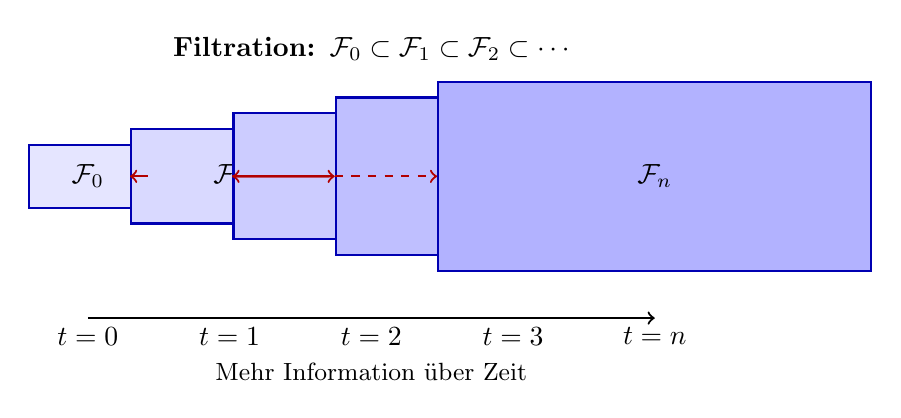
\begin{tikzpicture}[scale=0.9]
    % Zeitachse
    \draw[->, thick] (0,0) -- (8,0);
    \node[below] at (0,0) {$t=0$};
    \node[below] at (2,0) {$t=1$};
    \node[below] at (4,0) {$t=2$};
    \node[below] at (6,0) {$t=3$};
    \node[below] at (8,0) {$t=n$};
    
    % Filtration Boxen (wachsend)
    \node[rectangle, draw=blue!70!black, thick, minimum width=1.5cm, minimum height=0.8cm, fill=blue!10] (F0) at (0,2) {$\mathcal{F}_0$};
    \node[rectangle, draw=blue!70!black, thick, minimum width=2.5cm, minimum height=1.2cm, fill=blue!15] (F1) at (2,2) {$\mathcal{F}_1$};
    \node[rectangle, draw=blue!70!black, thick, minimum width=3.5cm, minimum height=1.6cm, fill=blue!20] (F2) at (4,2) {$\mathcal{F}_2$};
    \node[rectangle, draw=blue!70!black, thick, minimum width=4.5cm, minimum height=2.0cm, fill=blue!25] (F3) at (6,2) {$\mathcal{F}_3$};
    \node[rectangle, draw=blue!70!black, thick, minimum width=5.5cm, minimum height=2.4cm, fill=blue!30] (Fn) at (8,2) {$\mathcal{F}_n$};
    
    % Pfeile zeigen Wachstum
    \draw[->, thick, red!70!black] (F0) -- (F1);
    \draw[->, thick, red!70!black] (F1) -- (F2);
    \draw[->, thick, red!70!black] (F2) -- (F3);
    \draw[->, thick, red!70!black, dashed] (F3) -- (Fn);
    
    % Label
    \node[above] at (4, 3.5) {\textbf{Filtration: $\mathcal{F}_0 \subset \mathcal{F}_1 \subset \mathcal{F}_2 \subset \cdots$}};
    \node[below] at (4, -0.5) {\small Mehr Information über Zeit};
\end{tikzpicture}
\end{center}
\end{denoobification}

\begin{denoobification}[Adaptiert]
\textbf{Was bedeutet "adaptiert"?}

Ein Prozess $\{X_n\}$ heißt \textbf{adaptiert} an die Filtration $\{\mathcal{F}_n\}$, wenn $X_n$ für jedes $n$ $\mathcal{F}_n$-messbar ist.

\textbf{Intuition:} Zum Zeitpunkt $n$ kennen wir den Wert von $X_n$ bereits - er hängt nur von Information ab, die bis zum Zeitpunkt $n$ verfügbar ist.

\textbf{Beispiel:} Bei einem Random Walk $S_n = X_1 + \cdots + X_n$ ist $S_n$ adaptiert an $\mathcal{F}_n = \sigma(X_1, \ldots, X_n)$, weil $S_n$ nur von den ersten $n$ Schritten abhängt.

\textbf{$\star$ Mental Model zum Auswendiglernen:}
\begin{itemize}
    \item \textbf{Analogie:} "Adaptiert" = "passt sich an" - der Prozess verwendet nur Information, die bereits verfügbar ist
    \item \textbf{Merksatz:} "Adaptiert = $X_n$ hängt nur von $\mathcal{F}_n$ ab (keine Zukunft!)"
    \item \textbf{Test:} Können wir $X_n$ zum Zeitpunkt $n$ berechnen? Ja → adaptiert
    \item \textbf{Visualisierung:} Wie ein "Blindflug" - Sie können nur auf das schauen, was Sie bereits gesehen haben, nicht in die Zukunft
\end{itemize}
\end{denoobification}

\begin{denoobification}[Stoppzeit]
\textbf{Was ist eine Stoppzeit?}

Eine \textbf{Stoppzeit} $\tau$ ist eine Zufallsvariable $\tau: \Omega \to \{0, 1, 2, \ldots\} \cup \{\infty\}$, sodass für jedes $n$ das Ereignis $\{\tau \leq n\} \in \mathcal{F}_n$ liegt.

\textbf{Intuition:} Eine Stoppzeit ist ein "Stopp-Regel" - basierend auf der Information bis zum Zeitpunkt $n$ können wir entscheiden, ob wir bereits gestoppt haben ($\tau \leq n$).

\textbf{Beispiele:}
\begin{itemize}
    \item $\tau = 10$ (konstante Stoppzeit - immer bei 10 stoppen)
    \item $\tau = \inf\{n : S_n \geq 5\}$ (erste Zeit, wo Random Walk den Wert 5 erreicht)
    \item $\tau = \inf\{n : |S_n| \geq 10\}$ (erste Zeit, wo Random Walk den Abstand 10 vom Start hat)
\end{itemize}

\textbf{Wichtig:} Eine Stoppzeit darf \textit{nicht} von zukünftiger Information abhängen. Wir können nicht "bei der ersten Zeit stoppen, wo $S_{n+1} > 10$" sagen, weil wir $S_{n+1}$ zum Zeitpunkt $n$ noch nicht kennen.

\textbf{$\star$ Mental Model zum Auswendiglernen:}
\begin{itemize}
    \item \textbf{Analogie:} Eine Stoppzeit ist wie eine "Stopp-Regel" beim Spielen - basierend auf dem, was Sie bisher gesehen haben
    \item \textbf{Merksatz:} "Stoppzeit = Entscheidung basierend nur auf vergangener Information"
    \item \textbf{Test:} Können wir zum Zeitpunkt $n$ entscheiden, ob $\tau \leq n$? Ja → Stoppzeit
    \item \textbf{Visualisierung:} Wie ein "Stoppschild" - Sie sehen es, wenn Sie es erreichen, nicht bevor
\end{itemize}

\begin{center}
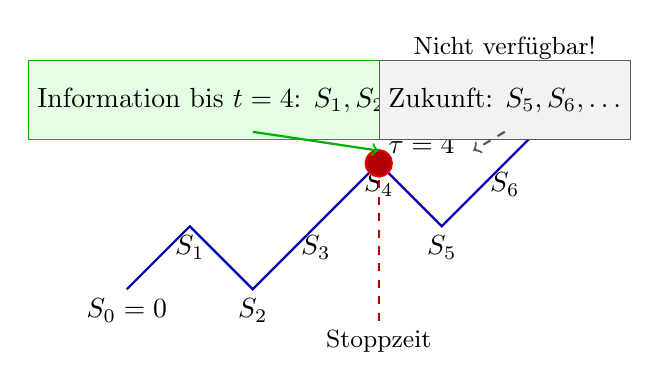
\begin{tikzpicture}[scale=0.8]
    % Random Walk Pfad
    \draw[thick, blue!70!black] (0,0) -- (1,1) -- (2,0) -- (3,1) -- (4,2) -- (5,1) -- (6,2) -- (7,3);
    \node[below] at (0,0) {$S_0=0$};
    \node[below] at (1,1) {$S_1$};
    \node[below] at (2,0) {$S_2$};
    \node[below] at (3,1) {$S_3$};
    \node[below] at (4,2) {$S_4$};
    \node[below] at (5,1) {$S_5$};
    \node[below] at (6,2) {$S_6$};
    \node[below] at (7,3) {$S_7$};
    
    % Stoppzeit markieren (z.B. erste Zeit wo S_n >= 2)
    \node[circle, fill=red!70!black, draw=red!90!black, thick, minimum size=0.3cm] at (4,2) {};
    \node[above right] at (4,2) {$\tau = 4$};
    \draw[red!70!black, dashed, thick] (4,2) -- (4,-0.5);
    \node[below] at (4,-0.5) {\small Stoppzeit};
    
    % Information verfügbar
    \node[rectangle, draw=green!70!black, fill=green!10, minimum width=4cm, minimum height=1cm] at (2,3) {Information bis $t=4$: $S_1, S_2, S_3, S_4$};
    \draw[->, green!70!black, thick] (2,2.5) -- (4,2.2);
    
    % Zukunft (nicht verfügbar)
    \node[rectangle, draw=gray!70!black, fill=gray!10, minimum width=3cm, minimum height=1cm] at (6,3) {Zukunft: $S_5, S_6, \ldots$};
    \draw[->, gray!70!black, dashed, thick] (6,2.5) -- (5.5,2.2);
    \node[above] at (6,3.5) {\small Nicht verfügbar!};
\end{tikzpicture}
\end{center}
\end{denoobification}

\vspace{0.5cm}

% ============================================
% MULTIPLE CHOICE FRAGEN
% ============================================

\subsection{Multiple-Choice Fragen zur Selbstkontrolle}

\begin{multiplechoice}
\textbf{Frage 1:} Was ist ein Wahrscheinlichkeitsraum $(\Omega, \mathcal{F}, \mathbb{P})$?

\begin{enumerate}[label=(\alph*)]
    \item Eine Menge von Zahlen
    \item Ein Tripel bestehend aus Ergebnismenge, $\sigma$-Algebra und Wahrscheinlichkeitsmaß
    \item Eine Funktion, die Wahrscheinlichkeiten berechnet
    \item Ein mathematisches Modell für deterministische Prozesse
\end{enumerate}

\begin{solution}
\textbf{Richtige Antwort: (b)}

Ein Wahrscheinlichkeitsraum ist ein Tripel $(\Omega, \mathcal{F}, \mathbb{P})$, wobei:
\begin{itemize}
    \item $\Omega$ die Ergebnismenge ist
    \item $\mathcal{F}$ eine $\sigma$-Algebra ist
    \item $\mathbb{P}$ ein Wahrscheinlichkeitsmaß ist
\end{itemize}

Dies ist das fundamentale Modell für Zufallsexperimente in der Wahrscheinlichkeitstheorie.
\end{solution}
\end{multiplechoice}

\begin{multiplechoice}
\textbf{Frage 2:} Was bedeutet es, dass ein Prozess $\{X_n\}$ an eine Filtration $\{\mathcal{F}_n\}$ adaptiert ist?

\begin{enumerate}[label=(\alph*)]
    \item $X_n$ hängt von zukünftigen Werten ab
    \item $X_n$ ist $\mathcal{F}_n$-messbar für alle $n$
    \item $X_n$ ist unabhängig von $\mathcal{F}_n$
    \item $X_n$ ist konstant
\end{enumerate}

\begin{solution}
\textbf{Richtige Antwort: (b)}

Ein Prozess ist adaptiert, wenn $X_n$ für jedes $n$ $\mathcal{F}_n$-messbar ist. Das bedeutet, dass der Wert von $X_n$ nur von Information abhängt, die bis zum Zeitpunkt $n$ verfügbar ist (beschrieben durch $\mathcal{F}_n$).
\end{solution}
\end{multiplechoice}

\begin{multiplechoice}
\textbf{Frage 3:} Welche der folgenden ist \textbf{keine} Stoppzeit?

\begin{enumerate}[label=(\alph*)]
    \item $\tau = 5$ (konstante Stoppzeit)
    \item $\tau = \inf\{n : S_n \geq 10\}$ (erste Zeit, wo $S_n \geq 10$)
    \item $\tau = \inf\{n : S_{n+1} > 0\}$ (erste Zeit, wo nächster Wert $> 0$)
    \item $\tau = \inf\{n : |S_n| \geq 5\}$ (erste Zeit, wo $|S_n| \geq 5$)
\end{enumerate}

\begin{solution}
\textbf{Richtige Antwort: (c)}

Option (c) ist keine Stoppzeit, weil sie von zukünftiger Information abhängt. Zum Zeitpunkt $n$ kennen wir $S_{n+1}$ noch nicht, daher können wir nicht entscheiden, ob $\tau \leq n$ gilt.

Die anderen Optionen sind gültige Stoppzeiten:
\begin{itemize}
    \item (a): Konstante Stoppzeit ist immer eine Stoppzeit
    \item (b): Basierend auf $S_1, \ldots, S_n$ können wir entscheiden, ob $S_n \geq 10$
    \item (d): Basierend auf $S_1, \ldots, S_n$ können wir entscheiden, ob $|S_n| \geq 5$
\end{itemize}
\end{solution}
\end{multiplechoice}

\begin{multiplechoice}
\textbf{Frage 4:} Was ist die Martingal-Eigenschaft?\\

\begin{enumerate}[label=(\alph*)]
    \item $\mathbb{E}[M_n] = 0$ für alle $n$
    \item $\mathbb{E}[M_{n+1} | \mathcal{F}_n] = M_n$ fast sicher
    \item $M_n$ ist konstant
    \item $\mathbb{E}[M_n^2] < \infty$ für alle $n$
\end{enumerate}

\begin{solution}
\textbf{Richtige Antwort: (b)}

Die Martingal-Eigenschaft ist $\mathbb{E}[M_{n+1} | \mathcal{F}_n] = M_n$ fast sicher. Das bedeutet: Die beste Vorhersage für den nächsten Wert $M_{n+1}$, gegeben die Information bis zum Zeitpunkt $n$, ist der aktuelle Wert $M_n$.

Intuitiv: Ein Martingal hat keine "Trend" - im Durchschnitt bleibt es gleich.
\end{solution}
\end{multiplechoice}

\begin{multiplechoice}
\textbf{Frage 5:} Was besagt das Optional Stopping Theorem?

\begin{enumerate}[label=(\alph*)]
    \item $\mathbb{E}[M_\tau] = \mathbb{E}[M_0]$ für alle Stoppzeiten $\tau$
    \item $\mathbb{E}[M_\tau] = \mathbb{E}[M_0]$ unter bestimmten Bedingungen (z.B. $\mathbb{E}[\tau] < \infty$)
    \item $M_\tau$ ist immer integrierbar
    \item Stoppzeiten existieren immer
\end{enumerate}

\begin{solution}
\textbf{Richtige Antwort: (b)}

Das Optional Stopping Theorem besagt, dass $\mathbb{E}[M_\tau] = \mathbb{E}[M_0]$ unter bestimmten Bedingungen gilt, z.B.:
\begin{itemize}
    \item $\tau$ ist beschränkt
    \item $\mathbb{E}[\tau] < \infty$ und $|M_{n+1} - M_n|$ ist beschränkt
    \item $M_\tau$ ist integrierbar und $\lim_{n \to \infty} \mathbb{E}[M_n \mathbf{1}_{\{\tau > n\}}] = 0$
\end{itemize}

Ohne diese Bedingungen kann das Theorem \textit{falsch} sein, wie die Boss Challenge zeigt!
\end{solution}
\end{multiplechoice}

\vspace{1cm}

% ============================================
% CHAPTER CONTENT
% ============================================

\section{Bedingte Erwartung}

Die bedingte Erwartung ist eines der fundamentalen Konzepte in der Wahrscheinlichkeitstheorie und bildet die Grundlage für die Martingal-Theorie.

\begin{definition}[Bedingte Erwartung]
Sei $(\Omega, \mathcal{F}, \mathbb{P})$ ein Wahrscheinlichkeitsraum, $\mathcal{G} \subset \mathcal{F}$ eine $\sigma$-Algebra, und $X$ eine integrierbare Zufallsvariable. Die \textbf{bedingte Erwartung} $\mathbb{E}[X | \mathcal{G}]$ ist die (fast sicher eindeutige) $\mathcal{G}$-messbare Zufallsvariable, die für alle $A \in \mathcal{G}$ erfüllt:

\begin{equation}
\int_A \mathbb{E}[X | \mathcal{G}] \, d\mathbb{P} = \int_A X \, d\mathbb{P}
\end{equation}
\end{definition}

\begin{theorem}[Eigenschaften der bedingten Erwartung]
Seien $X, Y$ integrierbare Zufallsvariablen und $\mathcal{G}, \mathcal{H}$ $\sigma$-Algebren. Dann gelten:

\begin{enumerate}
    \item \textbf{Linearität:} $\mathbb{E}[aX + bY | \mathcal{G}] = a\mathbb{E}[X | \mathcal{G}] + b\mathbb{E}[Y | \mathcal{G}]$ für $a, b \in \mathbb{R}$
    \item \textbf{Tower Property:} $\mathbb{E}[\mathbb{E}[X | \mathcal{G}] | \mathcal{H}] = \mathbb{E}[X | \mathcal{H}]$ wenn $\mathcal{H} \subset \mathcal{G}$
    \item \textbf{Monotonie:} Wenn $X \leq Y$ fast sicher, dann $\mathbb{E}[X | \mathcal{G}] \leq \mathbb{E}[Y | \mathcal{G}]$ fast sicher
    \item \textbf{Jensen's Ungleichung:} Wenn $\phi$ konvex ist, dann $\phi(\mathbb{E}[X | \mathcal{G}]) \leq \mathbb{E}[\phi(X) | \mathcal{G}]$
\end{enumerate}
\end{theorem}

\begin{example}
Sei $X$ eine Zufallsvariable und $\mathcal{G} = \sigma(Y)$ für eine andere Zufallsvariable $Y$. Dann ist $\mathbb{E}[X | Y]$ eine Funktion von $Y$, die durch die Radon-Nikodym-Dichte charakterisiert wird.
\end{example}

\section{Martingale}

\begin{definition}[Martingal]
Sei $(\Omega, \mathcal{F}, \mathbb{P})$ ein Wahrscheinlichkeitsraum und $\{\mathcal{F}_n\}_{n \geq 0}$ eine Filtration. Eine Folge von Zufallsvariablen $\{M_n\}_{n \geq 0}$ heißt \textbf{Martingal} bezüglich $\{\mathcal{F}_n\}$, wenn:

\begin{enumerate}
    \item $M_n$ ist $\mathcal{F}_n$-messbar für alle $n$ (adaptiert)
    \item $\mathbb{E}[|M_n|] < \infty$ für alle $n$ (integrierbar)
    \item $\mathbb{E}[M_{n+1} | \mathcal{F}_n] = M_n$ fast sicher für alle $n$ (Martingal-Eigenschaft)
\end{enumerate}
\end{definition}

\begin{definition}[Submartingal und Supermartingal]
\begin{itemize}
    \item Wenn $\mathbb{E}[M_{n+1} | \mathcal{F}_n] \geq M_n$, heißt $\{M_n\}$ ein \textbf{Submartingal}
    \item Wenn $\mathbb{E}[M_{n+1} | \mathcal{F}_n] \leq M_n$, heißt $\{M_n\}$ ein \textbf{Supermartingal}
\end{itemize}
\end{definition}

\begin{example}[Symmetrisches Random Walk]
Sei $\{X_n\}$ eine Folge unabhängiger Zufallsvariablen mit $\mathbb{P}(X_n = 1) = \mathbb{P}(X_n = -1) = 1/2$. Definiere $S_n = \sum_{k=1}^n X_k$ und $\mathcal{F}_n = \sigma(X_1, \ldots, X_n)$. Dann ist $\{S_n\}$ ein Martingal.
\end{example}

\begin{theorem}[Martingal-Transform]
Sei $\{M_n\}$ ein Martingal und $\{H_n\}$ eine vorhersehbare Folge (d.h. $H_n$ ist $\mathcal{F}_{n-1}$-messbar). Dann ist die Martingal-Transform
\begin{equation}
(H \cdot M)_n = \sum_{k=1}^n H_k (M_k - M_{k-1})
\end{equation}
ein Martingal, wenn $\mathbb{E}[|(H \cdot M)_n|] < \infty$ für alle $n$.
\end{theorem}

\section{Optional Sampling Theorem}

\begin{definition}[Stoppzeit]
Eine Zufallsvariable $\tau: \Omega \to \{0, 1, 2, \ldots\} \cup \{\infty\}$ heißt \textbf{Stoppzeit} bezüglich $\{\mathcal{F}_n\}$, wenn $\{\tau \leq n\} \in \mathcal{F}_n$ für alle $n$.
\end{definition}

\begin{theorem}[Optional Sampling Theorem]
Sei $\{M_n\}$ ein Martingal und $\tau, \sigma$ Stoppzeiten mit $\sigma \leq \tau \leq N$ für eine Konstante $N$. Dann gilt:

\begin{equation}
\mathbb{E}[M_\tau | \mathcal{F}_\sigma] = M_\sigma
\end{equation}

Insbesondere: $\mathbb{E}[M_\tau] = \mathbb{E}[M_0]$.
\end{theorem}

\begin{theorem}[Optional Stopping Theorem - Erweiterte Version]
Sei $\{M_n\}$ ein Martingal und $\tau$ eine Stoppzeit. Dann gilt $\mathbb{E}[M_\tau] = \mathbb{E}[M_0]$, wenn eine der folgenden Bedingungen erfüllt ist:

\begin{enumerate}
    \item $\tau$ ist beschränkt (d.h. $\tau \leq N$ für eine Konstante $N$)
    \item $\mathbb{E}[\tau] < \infty$ und $|M_{n+1} - M_n| \leq K$ für eine Konstante $K$
    \item $M_\tau$ ist integrierbar und $\lim_{n \to \infty} \mathbb{E}[M_n \mathbf{1}_{\{\tau > n\}}] = 0$
\end{enumerate}
\end{theorem}

\section{Martingal-Konvergenzsatz}

\begin{theorem}[Martingal-Konvergenzsatz]
Sei $\{M_n\}$ ein Submartingal mit $\sup_n \mathbb{E}[M_n^+] < \infty$. Dann existiert eine Zufallsvariable $M_\infty$ mit $\mathbb{E}[|M_\infty|] < \infty$, sodass:

\begin{equation}
M_n \to M_\infty \quad \text{fast sicher für } n \to \infty
\end{equation}
\end{theorem}

\begin{corollary}
Jedes beschränkte Martingal konvergiert fast sicher gegen eine integrierbare Zufallsvariable.
\end{corollary}

\begin{theorem}[$L^p$-Konvergenz]
Sei $\{M_n\}$ ein Martingal. Wenn $\sup_n \mathbb{E}[|M_n|^p] < \infty$ für $p > 1$, dann konvergiert $\{M_n\}$ in $L^p$ gegen $M_\infty$.
\end{theorem}

\section{Quadratintegrierbare Martingale}

\begin{definition}[Quadratintegrierbares Martingal]
Ein Martingal $\{M_n\}$ heißt \textbf{quadratintegrierbar}, wenn $\mathbb{E}[M_n^2] < \infty$ für alle $n$.
\end{definition}

\begin{theorem}[Doob-Zerlegung]
Jedes Submartingal $\{X_n\}$ kann eindeutig geschrieben werden als:

\begin{equation}
X_n = M_n + A_n
\end{equation}

wobei $\{M_n\}$ ein Martingal ist und $\{A_n\}$ ein vorhersehbares, wachsendes Prozess mit $A_0 = 0$.
\end{theorem}

\begin{definition}[Quadratische Variation]
Für ein quadratintegrierbares Martingal $\{M_n\}$ definieren wir die \textbf{quadratische Variation}:

\begin{equation}
[M]_n = \sum_{k=1}^n (M_k - M_{k-1})^2
\end{equation}

und den \textbf{vorhersehbaren quadratischen Prozess}:

\begin{equation}
\langle M \rangle_n = \sum_{k=1}^n \mathbb{E}[(M_k - M_{k-1})^2 | \mathcal{F}_{k-1}]
\end{equation}
\end{definition}

\section{Integrale bezüglich Random Walk}

Sei $\{S_n\}$ ein symmetrischer Random Walk und $\{H_n\}$ eine vorhersehbare Folge. Das \textbf{stochastische Integral} ist definiert als:

\begin{equation}
(H \cdot S)_n = \sum_{k=1}^n H_k (S_k - S_{k-1}) = \sum_{k=1}^n H_k X_k
\end{equation}

wobei $X_k = S_k - S_{k-1}$ die Inkremente sind.

\begin{theorem}
Das stochastische Integral $(H \cdot S)_n$ ist ein Martingal, wenn $\mathbb{E}[|(H \cdot S)_n|] < \infty$ für alle $n$.
\end{theorem}

\begin{example}[Trading-Strategie]
In einem Finanzmarkt kann $H_n$ als die Anzahl der gehaltenen Aktien zum Zeitpunkt $n$ interpretiert werden, und $(H \cdot S)_n$ ist der Gewinn/Verlust der Strategie.
\end{example}

\section{Eine maximale Ungleichung}

\begin{theorem}[Doob's maximale Ungleichung]
Sei $\{M_n\}$ ein nicht-negatives Submartingal. Dann gilt für alle $\lambda > 0$:

\begin{equation}
\lambda \mathbb{P}\left(\max_{0 \leq k \leq n} M_k \geq \lambda\right) \leq \mathbb{E}[M_n]
\end{equation}
\end{theorem}

\begin{theorem}[Doob's $L^p$-Ungleichung]
Sei $\{M_n\}$ ein Martingal oder nicht-negatives Submartingal. Dann gilt für $p > 1$:

\begin{equation}
\mathbb{E}\left[\left(\max_{0 \leq k \leq n} |M_k|\right)^p\right] \leq \left(\frac{p}{p-1}\right)^p \mathbb{E}[|M_n|^p]
\end{equation}
\end{theorem}

\begin{corollary}
Für ein quadratintegrierbares Martingal $\{M_n\}$ gilt:

\begin{equation}
\mathbb{E}\left[\max_{0 \leq k \leq n} M_k^2\right] \leq 4 \mathbb{E}[M_n^2]
\end{equation}
\end{corollary}

\section{Übungen}

\begin{exercise}
Zeigen Sie, dass wenn $\{M_n\}$ ein Martingal ist, dann ist $\{M_n^2\}$ ein Submartingal.
\end{exercise}

\begin{exercise}
Sei $\{X_n\}$ eine Folge unabhängiger, identisch verteilter Zufallsvariablen mit $\mathbb{E}[X_1] = 0$ und $\text{Var}(X_1) = \sigma^2 < \infty$. 
Zeigen Sie, dass $\{S_n^2 - n\sigma^2\}$ ein Martingal ist, wobei $S_n = \sum_{k=1}^n X_k$.
\end{exercise}

\begin{exercise}
Beweisen Sie das Optional Sampling Theorem für beschränkte Stoppzeiten.
\end{exercise}

\begin{exercise}
Sei $\{M_n\}$ ein Martingal mit $\sup_n \mathbb{E}[M_n^2] < \infty$. Zeigen Sie, dass $\{M_n\}$ in $L^2$ konvergiert.
\end{exercise}

\begin{exercise}[Boss Challenge - Erweiterte Version]
Lösen Sie die Boss Challenge am Anfang dieses Kapitels. Konstruieren Sie explizit ein Gegenbeispiel für das Optional Stopping Theorem, wenn die Bedingung $\mathbb{E}[\tau] < \infty$ nicht erfüllt ist.
\end{exercise}

\section{Visualisierungen und Computerexperimente}

In diesem Abschnitt zeigen wir Visualisierungen, die mit den Python-Programmen aus dem \texttt{code/}-Verzeichnis erstellt wurden. Diese helfen dabei, die abstrakten Konzepte zu verstehen.

\subsection{Symmetrischer Random Walk}

\begin{figure}[h]
\centering

\includegraphics[width=0.9\textwidth]{random_walk_analysis.png}
\caption{Analyse des symmetrischen Random Walk: (oben links) Einzelne Pfade, (oben rechts) Erwartungswert $E[S_n] = 0$, (unten links) Varianz $Var(S_n) = n$, (unten rechts) Verteilung zu verschiedenen Zeitpunkten.}
\label{fig:random_walk}
\end{figure}

Die Abbildung~\ref{fig:random_walk} zeigt typische Pfade eines symmetrischen Random Walk. Man erkennt:
\begin{itemize}
    \item Der Erwartungswert bleibt bei $0$ (Martingal-Eigenschaft)
    \item Die Varianz wächst linear mit der Zeit: $Var(S_n) = n$
    \item Die Verteilung wird mit der Zeit breiter (Zentraler Grenzwertsatz)
\end{itemize}

\subsection{Martingal-Transform}

\begin{figure}[h]
\centering

\includegraphics[width=0.9\textwidth]{martingale_transform.png}
\caption{Martingal-Transform: (oben links) Basis-Martingal, (oben rechts) Transform mit konstanter Strategie $H_k = 1$, (unten links) Transform mit proportionaler Strategie $H_k = S_{k-1}$, (unten rechts) Vergleich der Erwartungswerte.}
\label{fig:martingale_transform}
\end{figure}

Abbildung~\ref{fig:martingale_transform} illustriert, wie verschiedene Strategien $H$ das Martingal transformieren. 
Wichtig: Alle Transforms bleiben Martingale (Erwartungswert bleibt konstant).

\subsection{Quadratische Variation}

\begin{figure}[h]
\centering

\includegraphics[width=0.9\textwidth]{quadratic_variation.png}
\caption{Quadratische Variation: (oben links) Martingal-Pfade, (oben rechts) Quadratische Variation $[M]_n$, (unten links) Vorhersehbarer quadratischer Prozess $\langle M \rangle_n$, (unten rechts) Verteilung von $[M]_{100}$.}
\label{fig:quadratic_variation}
\end{figure}

Die quadratische Variation $[M]_n$ misst die "Volatilität" des Martingals. Für einen symmetrischen Random Walk gilt $[M]_n = n$ (siehe Abbildung~\ref{fig:quadratic_variation}).

\subsection{Optional Stopping Theorem}

\begin{figure}[h]
\centering

\includegraphics[width=0.9\textwidth]{optional_stopping.png}
\caption{Optional Stopping Theorem: (oben links) Verteilung der Stoppzeiten, (oben rechts) Vergleich $E[X_0]$ vs $E[X_\tau]$, (unten links) Pfade mit markierten Stoppzeiten, (unten rechts) Unterschied $E[X_\tau] - E[X_0] \approx 0$.}
\label{fig:optional_stopping}
\end{figure}

Abbildung~\ref{fig:optional_stopping} zeigt, dass das Optional Stopping Theorem für beschränkte Stoppzeiten gilt: $E[X_\tau] = E[X_0] = 0$.

\subsection{Boss Challenge Visualisierung}

\begin{figure}[h]
\centering

\includegraphics[width=0.9\textwidth]{boss_challenge_visualization.png}
\caption{Boss Challenge: Der Martingal-Dämon. Vergleich zwischen beschränkter und unbeschränkter Stoppzeit. Die Visualisierung zeigt, warum das Optional Stopping Theorem für unbeschränkte Stoppzeiten im Allgemeinen nicht gilt.}
\label{fig:boss_challenge}
\end{figure}

Die Abbildung~\ref{fig:boss_challenge} visualisiert die Boss Challenge. Man sieht deutlich den Unterschied zwischen beschränkten und unbeschränkten Stoppzeiten.

\subsection{Python-Code für eigene Experimente}

Um diese Visualisierungen selbst zu erstellen oder eigene Experimente durchzuführen, verwenden Sie die Python-Programme im \texttt{code/chapter01/}-Verzeichnis:

\begin{verbatim}
# Beispiel: Symmetrischer Random Walk
from martingales import SymmetricRandomWalk

rw = SymmetricRandomWalk(n_steps=100, n_paths=1000, seed=42)
paths = rw.simulate()

# Berechne Statistiken
print(f"E[S_0] = {rw.mean(0)}")
print(f"E[S_100] = {rw.mean(100)}")
print(f"Var(S_100) = {rw.variance(100)}")
\end{verbatim}

Weitere Beispiele finden Sie in \texttt{example\_usage.py} und im Jupyter Notebook 
\texttt{Chapter01\_Notebook.ipynb}.
